\documentclass{standalone}
\usepackage{tkz-fct}
\usepackage{tkz-euclide}
\usepackage{color}
\renewcommand*\familydefault{\sfdefault}
\usepackage{sansmath}
\sansmath
\definecolor{gray75}{gray}{0.75}
\begin{document}
 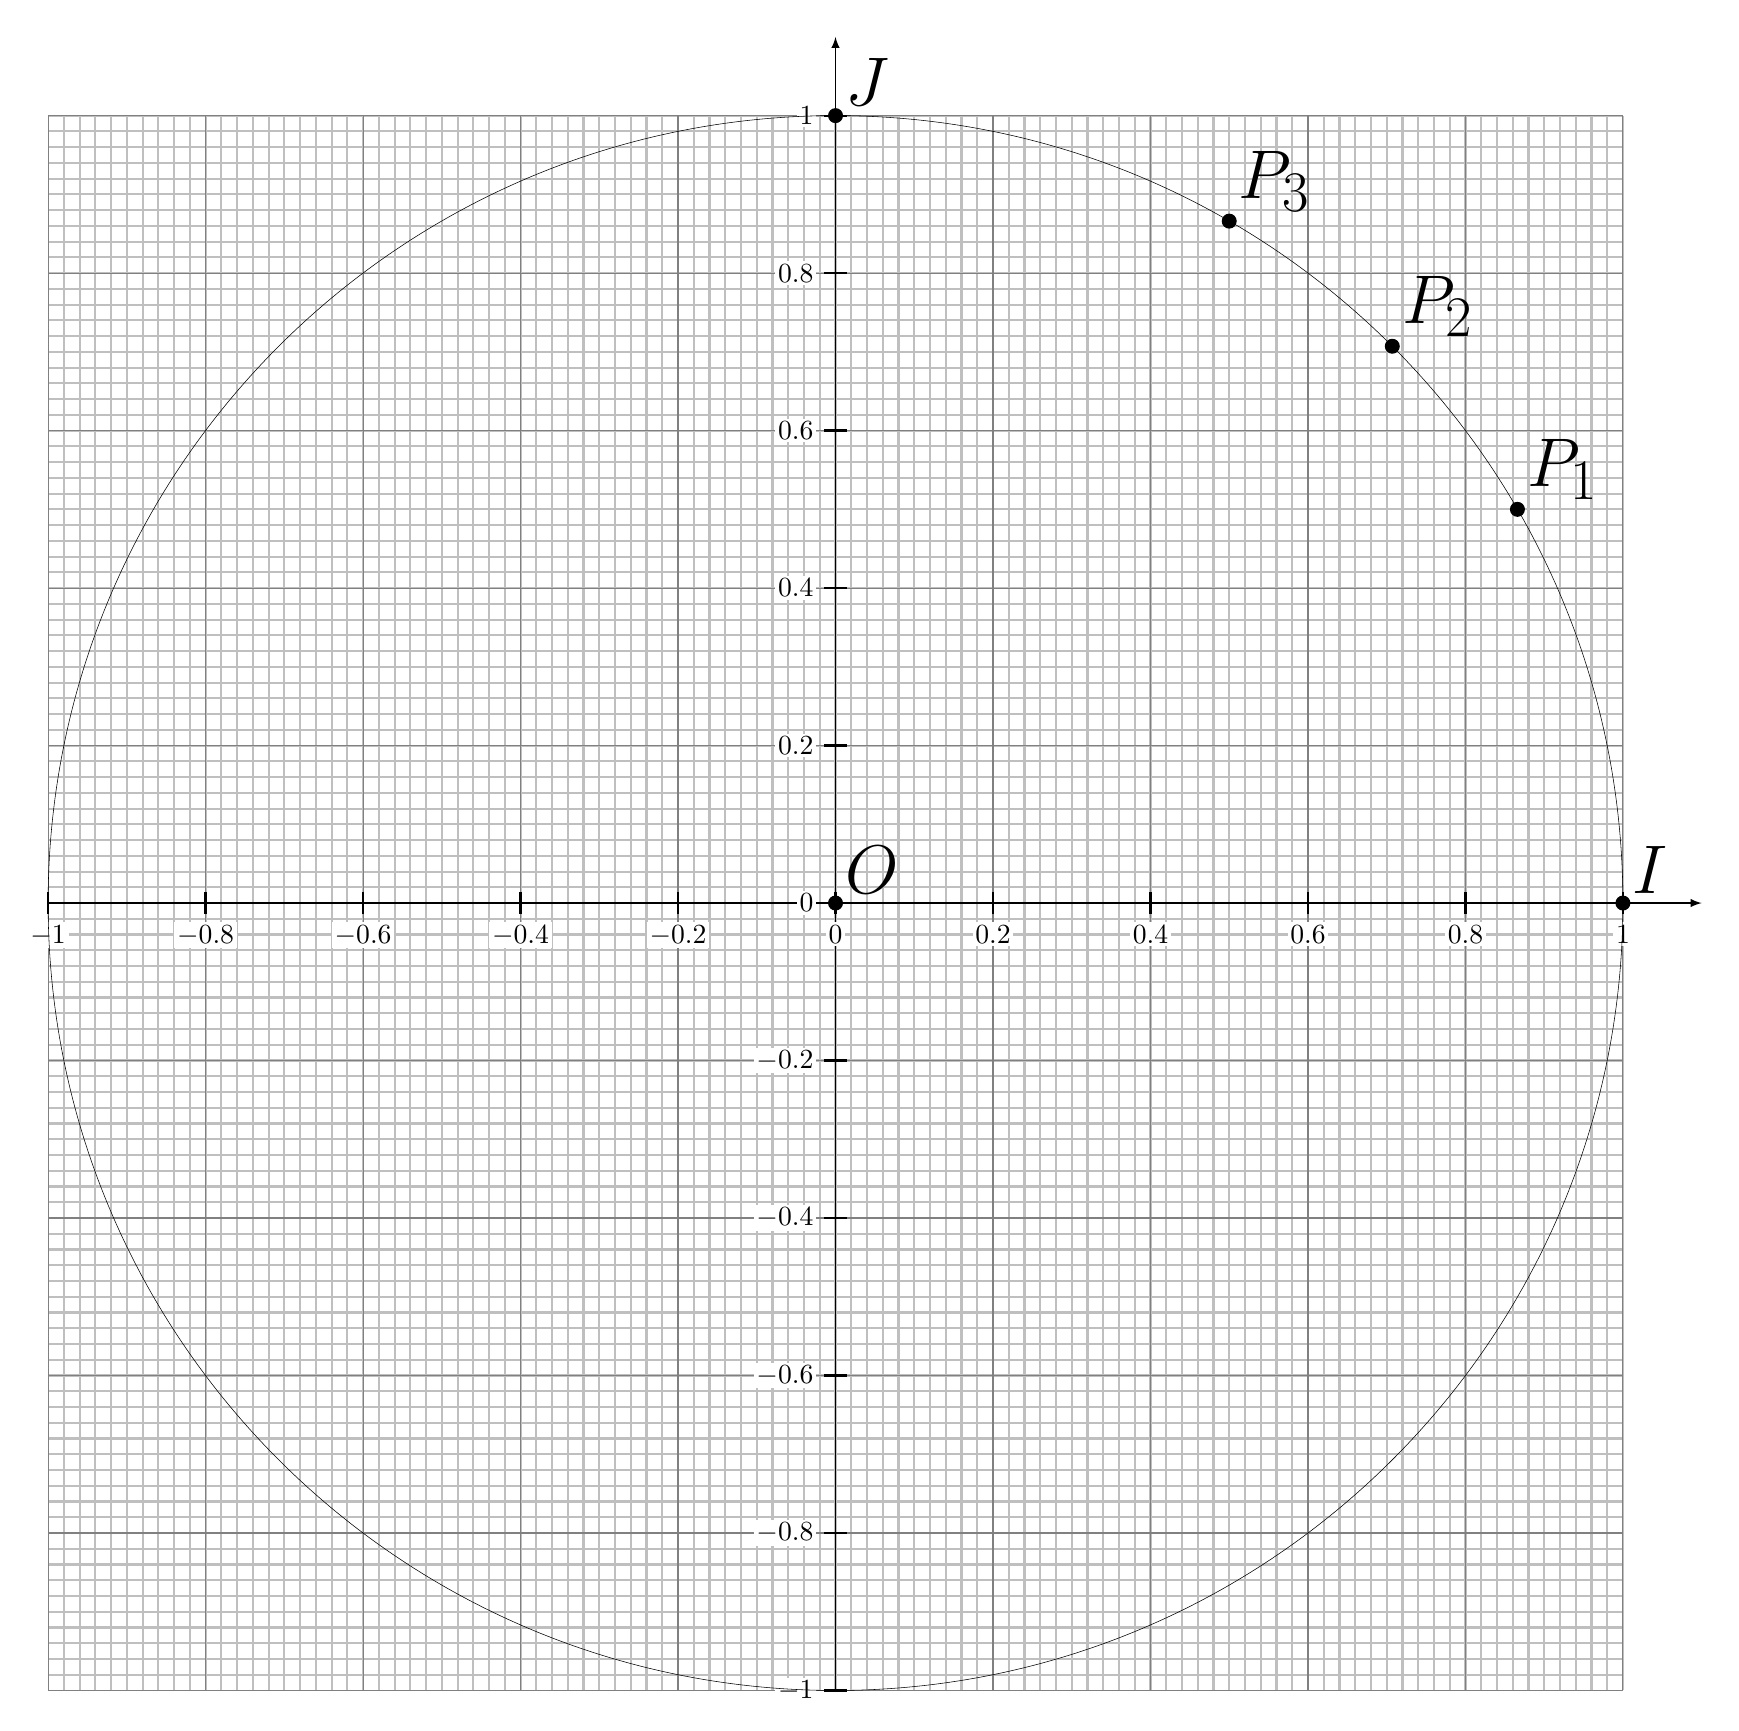
\begin{tikzpicture}[scale=2]
   \tkzInit[xmax=1.,ymax=1.,xmin=-1. ,ymin=-1,xstep=0.2,ystep=0.2]
   
   \begin{scope}
     \tkzGrid[sub,subxstep=0.02,subystep=0.02]
   \end{scope}
   \tkzAxeXY[label={}]
   \tkzDefPoints{0/0/O,0/1/A,1/0/I, 0/1/J}
   \tkzDrawCircle[color=black](O,A)
   \tkzDefShiftPoint[O](30:5){P1}
   \tkzDefShiftPoint[O](45:5){P2}
   \tkzDefShiftPoint[O](60:5){P3}
   \tkzDrawPoints[size=5pt](O,I,J,P1,P2,P3)
   \tkzLabelPoint[above right](P1){\Huge$P_1$}
   \tkzLabelPoint[above right](P2){\Huge$P_2$}
   \tkzLabelPoint[above right](P3){\Huge$P_3$}
   \tkzLabelPoint[above right](I){\Huge$I$}
   \tkzLabelPoint[above right](J){\Huge$J$}
   \tkzLabelPoint[above right](O){\Huge$O$}

\end{tikzpicture}
\end{document}
